\pagebreak
\section{РАЗРАБОТКА ПРОГРАММНЫХ МОДУЛЕЙ}
\label{sec:dev}

В данном разделе рассмотрим основные детали реализации системных вызовов и
пользовательских программ. Ввиду того, что одним важнейшими аспектами разработки
ядра является стабильность, этим вещам необходимо уделить особое внимание.
Однако, перед этим важно описать общие аспекты реализации поставленных задач при
добавлении системных вызовов.

Ранее в Linux все функции-обработчики системных вызовов традиционно имели
название вида \texttt{sys\_*}, например, вызов \texttt{read()} имел следующее
определение:
\medskip
\begin{lstlisting}[style=cstyle]
asmlinkage ssize_t sys_read(unsigned int fd, char __user * buf, size_t count)
\end{lstlisting}
\medskip

Тег \texttt{asmlinkage} сообщает компилятору, что функция не должна брать свои
аргументы из регистров, а должна использовать для этого стек. Все системные
вызовы отмечены тегом \texttt{asmlinkage}, так как долгое время вызов
обработчиков из таблицы \texttt{sys\_call\_table} осуществлялся напрямую из кода
на ассемблере.

Однако, в 2009-м году способ объявления обработчика изменился, и начиная с
версии 2.6.29 для этих целей используется набор из нескольких макросов
\texttt{SYSCALL\_DEFINE*}, из-за чего реализация того же вызова \texttt{read()}
сейчас выглядит так:
\medskip
\begin{lstlisting}[style=cstyle]
SYSCALL_DEFINE3(read, unsigned int, fd, char __user *, buf, size_t, count)
\end{lstlisting}
\medskip

Макрос \texttt{SYSCALL\_DEFINE3()} объявляет реализацию системного вызова
\texttt{read()} с тремя аргументами. При этом используется достаточно необычное
определение аргументов. Имена аргументов и их типы разделяются таким образом для
того, чтобы препроцессор Си мог осуществлять сопоставление аргументов по
бинарному интерфейсу системных вызовов с тем, что ожидает нормальная функция на
Си. Далее будем рассматривать реализацию вызов в архитектуре x86\_64, как
наиболее популярной в данный момент, после нескольких раскрытий макросов, строка
\texttt{SYSCALL\_DEFINE3()} превращается в следующее:
\medskip
\begin{lstlisting}[style=cstyle]
asmlinkage long sys_read(int fd, char __user *buf, size_t
count) __attribute__((alias(__stringify(SyS_read))));
asmlinkage long SyS_read(long fd, long buf, long count)
{
	long ret = SYSC_read((int) fd, (char __user *) buf, (size_t) count);
	return ret;
}
static inline SYSC_read(int fd, char __user *buf, size_t count)
\end{lstlisting}
\medskip

Как видно, описываются две разные функции и один псевдоним функции.
\texttt{SyS\_read()} объявляется с атрибутом asmlinkage и с теми же аргументами,
но объявленными c типом \texttt{long}, который всегда соответствует размеру
регистра~--- в том виде, как непосредственно передаются аргументы из
пользовательского пространства. Эта функция приводит аргументы в ожидаемые типы,
а после вызывает \texttt{SYSC\_read()}, которая является настоящим именем
функции, содержащей код, реализующий системный вызов. При этом, функция
объявлена как \texttt{static} \texttt{inline}, поэтому она будет заменена
непосредственно на \texttt{SyS\_read()}.

Именно указатель на функцию \texttt{SyS\_read()} помещается в соответствующее
место в массиве \texttt{sys\_call\_table}, а вызов непосредственно нужного
обработчика сводится к выбору указателя по индексу:
\medskip
\begin{lstlisting}[style=cstyle]
if (likely ((nr & __SYSCALL_MASK) < NR_syscalls)) {
	nr = array_index_nospec (nr & __SYSCALL_MASK, NR_syscalls);
	regs->ax = sys_call_table[nr](
		regs->di, regs->si, regs->dx,
		regs->r10, regs->r8, regs->r9);
}
\end{lstlisting}
\medskip

Использование \texttt{array\_index\_nospec()} запрещает процессору осуществить
вызов спекулятивно, тем самым блокируя любые попытки вызовов по адресу вне
\texttt{sys\_call\_table}. Такие меры необходимы для обхода аппаратной
уязвимости Spectre. Непосредственно макросы-обертки при объявлении обработчиков
используются для покрытия уязвимости CVE-2009-0029, позволяющей заполнять
регистр с 32-битный аргументом 64-битным значением, что давало возможность
выходить за пределы массивов при адресации. В связи с этим ядро и производит
дополнительное приведение типов в макросах, описанное выше.

При написании любого кода ядра необходимо учитывать факторы окружения. В любое
время каждый из процессоров в системе может быть в различных состояниях:
\begin{itemize}
\item не связан с каким-либо процессом и обрабатывает аппаратное прерывание;
\item обслуживает программные прерывания;
\item исполняет код в пространстве ядра, связанный с процессом, то есть
  исполняется в пользовательском контексте;
\item исполняет код пространства пользователя.
\end{itemize}

Между этими состояниями имеется очередность. Различные контексты пользователя,
как в пространстве ядра, так и в пространстве пользователя, могут вытеснять друг
друга, однако с прерываниями имеется строгая иерархия. В то время как
исполняется обработчик программного прерывания, ни один другой такой обработчик
этого же типа не будет его вытеснять, а аппаратное прерывание вытеснить может.
Существует несколько способов, которыми пользовательский контекст может
блокировать прерывания, что будет описано ниже. Поэтому стоит учитывать данные
факторы. Кроме того, существует несколько особенностей в работе кода ядра:
\begin{itemize}
\item нет защиты памяти. Если повредится память, как в контексте пользователя,
  так и в контексте прерывания, вся машина может выйдет из строя;
\item нельзя использовать операции с плавающей запятой или MMX. Контекст
  сопроцессора для операций с плавающей точкой не сохраняется из-за больших
  временных затрат на такие действия. Существует только несколько исключений в
  коде ядра, к которых ввиду слишком долгого исполнения криптографических
  алгоритмов используются векторные вычисления и сохраняется весь контекст
  исполняющего устройства;
\item жесткий предел стека. В зависимости от параметров конфигурации стек ядра
  составляет от трех до шести килобайт на большинстве 32-битных и 14 килобайт
  для большинства 64-битных архитектур, и часто используется в том числе
  прерываниями, поэтому не рекомендуется использовать весь стек. Следует избегать
  глубокой рекурсии и больших локальных массивов в стеке, вместо этого следует
  выделять их динамически;
\item в коде ядра нужно избегать использования платформозависимых вещей, и
  оставлять их только там, где это необходимо, так как, например, сборка для
  встроенного устройства должна быть полностью минимизирована. Как правило,
  подобный код должен быть расположен в архитектурно зависимой директории ядра.
\end{itemize}

Важным моментом является порядок вызова спящих и не спящих функций. Нельзя
вызывать какие-либо спящие функции, за исключением случаев, когда:
\begin{itemize}
\item код исполняется в контексте пользователя;
\item в коде нет спинлоков.
\end{itemize}

Следует обратить внимание, что некоторые функции могут спать неявно, например,
функции доступа к пространству пользователя (так как, например, память по
переданному указателю может быть отображена в файл на сетевой файловой системе)
или функции выделения ядерной памяти без флага \texttt{GFP\_ATOMIC}. В качестве
вспомогательного средства в этом вопросе можно использовать опцию компиляции
\texttt{CONFIG\_DEBUG\_ATOMIC\_SLEEP}, и ядро предупредит в случае нарушения
правил работы с памятью.

% pidmap

Как уже было сказано в разделе \ref{sec:func}, вызов \texttt{sys\_pidmap} может
возвращать в пространство пользователя идентификаторы разных задач в зависимости
от переданных флагов. В связи с этим логично разделить код вызова не несколько
функций в самом начале по функциональному критерию. Кроме того, так как один из
флагов является опциональным дополнением к некоторым другим, важно отделить
решающие параметры от остальных:
\medskip
\begin{lstlisting}[style=cstyle]
int param = flags & PIDMAP_PARAM;
switch (param) {
case PIDMAP_TASKS:
case PIDMAP_PROC:
	return pidmap_tasks(pids, count, start, flags);
case PIDMAP_CHILDREN:
	return pidmap_children(pid, pids, count, start);
case PIDMAP_THREADS:
	return pidmap_threads(pid, pids, count, start);
}
\end{lstlisting}
\medskip

В данном случае \texttt{PIDMAP\_PARAM}~--- маска, оставляющая только те биты, в
одном из которых должен находиться флаг, описывающий необходимое поведение. У
добавленных функций следующие назначения:
\begin{itemize}
\item \texttt{pidmap\_tasks}~--- предоставление всех процессов или потоков в системе;
\item \texttt{pidmap\_children}~--- предоставление списка детей определенного процесса;
\item \texttt{pidmap\_threads}~--- предоставление списка потоков процесса.
\end{itemize}

Так как флаги \texttt{PIDMAP\_TASKS} и \texttt{PIDMAP\_PROC} дают общесистемную
информацию, параметр \texttt{pid} системного вызова игнорируется. Кроме того,
оба флага используют одну функцию ввиду того, что ее реализации используется
проход по массиву выделенных идентификаторов и уже в процессе прохода
определяется, нужен ли пользователю идентификатор.

В функции \texttt{pidmap\_tasks} существует возможность оптимизации процесса
получения идентификаторов. Дело в том, что ввиду поддержки ядром UNIX
Timesharing System процессы существуют в пределах своего пространства имен.
Пространство имен идентификаторов процессов описывается структурой
\texttt{pid\_namespace}:
\medskip
\begin{lstlisting}[style=cstyle]
struct pid_namespace {
	struct kref kref;
	struct pidmap pidmap[PIDMAP_ENTRIES];
	struct rcu_head rcu;
	int last_pid;
	/* ... */
}
\end{lstlisting}
\medskip

Данная структура управляет областью видимости процессов, процессом выделения
идентификаторов. Как видно, идентификаторы выделяются при помощи массива
структур \texttt{pidmap} в одном из полей структуры пространства имен.
Определение структуры следующее:
\medskip
\begin{lstlisting}[style=cstyle]
struct pidmap {
       atomic_t nr_free;
       void *page;
};
\end{lstlisting}
\medskip

Структура описывает маску выделенных идентификаторов, в ней содержится поле с
числом свободных идентификаторов \texttt{nr\_free}, а также указатель на
страницу с непосредственно битовой маской \texttt{page}. Единичный бит означает,
что идентификатор выделен, нулевой~--- свободен. В массиве указателей
\texttt{pidmap} некоторые элементы могут быть нулевыми, то есть страница
может быть не выделена для экономии памяти.

Таким образом, поиск идентификаторов заключается в проходе по массиву страниц с
битовыми масками, а само значение идентификатора складывается из номера
структуры, номера числа в странице и номера байта в числе. Поиске очередного
бита осуществляется с помощью функции \texttt{\_\_ffs()}, которая на большинстве
архитектур компилируется в машинную инструкцию \texttt{ffs} (find first set), с
помощью которой определяется номер первого ненулевого бита в числе.

Функции \texttt{pidmap\_children} и \texttt{pidmap\_threads} предназначены
соответственно для получения идентификаторов дочерних процессов и потоков
процесса. Обе функции в первую очередь должны получить структуру, описывающую
процесс с переданным в системный вызов идентификатором. Кроме того, хорошим
решением в данном случае является возможность более быстрого и удобного указания
процессом на себя путем передачи идентификатора, равного единице. Часто в
различных источниках процессом с нулевым идентификатором называют само ядро
системы, однако это не так. Технически, задачей с нулевым идентификатором
является так называемая задача \texttt{init\_task}, статически существующая в
ядре и исполняемом файле с секции \texttt{.data}. Эта задача фактически фиктивна
и существует только ради поддержки факта того, что у каждого процесса должен
быть существующий родитель, чтобы все процессы таким образом образовывали
дерево, и фиктивная начальная задача является в таком дереве корнем.

Логичным решением ввиду аналогичности процесса получения исследуемого процесса
является выделение этого действия в отдельную функцию \texttt{pidmap\_get\_task}
для уменьшения повторяемости кода и поддерживаемости. Определение функции
следующее:
\medskip
\begin{lstlisting}[style=cstyle]
static struct task_struct *pidmap_get_task(pid_t pid, bool *has_perms);
\end{lstlisting}
\medskip

Получение указателя на структуру, описывающую текущую задачу, осуществляется при
помощи макроса \texttt{current}, результат которого разнится между контекстами.
Так как Linux поддерживает пространства имен в соответствии с Unix Timesharing
System, важно получить доступ к пространству идентификаторов процессов
относительно текущего процесса, искать процесс относительно этого пространства
имен, а также проверить наличие прав на доступ к информации для текущего
процесса. Получение текущего пространства осуществляется при помощи функции
\texttt{task\_active\_pid\_ns()} с передачей параметром \texttt{current}.
Получение указателя на структуру задачи по идентификатору и пространству имен
выполняется при помощи вызова функции \texttt{find\_task\_by\_pid\_ns()},
которой передаются указатели на структуру задачи и структуру пространства имен
идентификаторов процессов. Основная часть получения задачи выглядит следующим
образом:
\medskip
\begin{lstlisting}[style=cstyle]
if (pid == 0) {
	*has_perms = true;
	return current;
}

pid_ns = task_active_pid_ns(current);
task = find_task_by_pid_ns(pid, pid_ns);
if (!task)
	return ERR_PTR(-ESRCH);
*has_perms = pidmap_perm(pid_ns);
if (!*has_perms && !ptrace_may_access(task, PTRACE_MODE_READ_FSCREDS))
	return ERR_PTR(-EACCES);
\end{lstlisting}
\medskip

Функция \texttt{pidmap\_perm} предназначена для проверки у пространства имен
наличия параметра \texttt{HIDEPID\_INVISIBLE}. Данный параметр предназначен для
сокрытия от задачи всех других процессов, другими словами, в директории
\texttt{/proc/} процесс обнаружит из директорий с информацией о процессах
только свою директорию о себе. Проверка осуществлена в данном виде:
\medskip
\begin{lstlisting}[style=cstyle]
static inline bool pidmap_perm(const struct pid_namespace *pid_ns)
{
	return pid_ns->hide_pid < HIDEPID_INVISIBLE
		|| in_group_p(pid_ns->pid_gid);
}
\end{lstlisting}
\medskip

Функция \texttt{ERR\_PTR()} используется в случаях, когда функция может
возвратить либо указатель, либо ошибку. Для подобного опционального возврата
не используется дополнительных структур или выделений памяти. Вместо этого
используется факт того, что несколько десятков верхних адресов никогда не могут
быть валидными, поэтому их можно использовать в качестве кода ошибки. Упомянутая
функция используется для упаковки ошибки в адрес. Кроме нее, используются такие
функции как \texttt{IS\_ERR()} для проверки возвращенного функцией указателя на
наличие в нем кода ошибки, \texttt{IS\_ERR()} для получения кода ошибки из
возвращенного указателя и другие. Типичный сценарий использования выглядит
следующим образом:
\medskip
\begin{lstlisting}[style=cstyle]
rcu_read_lock();
task = pidmap_get_task(pid, &has_perms);
if (IS_ERR(task)) {
	/* Returned error */
	rcu_read_unlock();
	return PTR_ERR(task);
}
\end{lstlisting}
\medskip

После получения структуры исследуемого процесса функциям необходимо
проитерироваться по дочерним процессам либо потокам, в зависимости от того,
какая выполняется функция.

Сама по себе задача представлена структурой \texttt{task\_struct}, которая
является одной из самых больших структур ядра. В ней расположена различная
информация для планировщика, состояние, флаги, идентификаторы и различная другая
информация, указатели на структуры, описывающие виртуальную память, файловую
подсистему, а также структуры элементов списков.

Структуры в ядре Linux объединены в списки несколько иным образом по сравнению с
тем, как это делают в программах пространства пользователя. Фактически, списки в
ядре представляют собой кольца. При этом, вместо того, чтобы иметь в специальном
месте указатель на начало списка, каждый элемент является головой списка. Кроме
того, структуры, описывающие элемент списка (содержащие указатели на соседей),
находятся внутри структур, живущих в списках, а не наоборот, когда в структуре
элемента списка был указатель на настоящую структуру, к которой предоставляется
доступ. Эта структура имеет следующий вид:
\medskip
\begin{lstlisting}[style=cstyle]
struct list_head {
	struct list_head *next, *prev;
};
\end{lstlisting}
\medskip

Пара указателей содержат адреса аналогичных структур в объектах-соседях, а
доступ к самим объектам осуществляется при помощи использования нестандартной
возможности времени компиляции \texttt{offsetof}, позволяющей получить смещение
поля в структуре, после чего полученной смещение можно вычесть из виртуального
адреса структуры \texttt{list\_head} для получения адреса содержащей ее
структуры. Естественно, что постоянное ручное использование подобной адресной
арифметики способно вызвать большое количество ошибок, поэтому для списков
существует множество макросов, упрощающих их использование:
\medskip
\begin{lstlisting}[style=cstyle]
#define list_entry(ptr, type, member) \
	container_of(ptr, type, member)
#define container_of(ptr, type, member) ({		\
	void *__mptr = (void *)(ptr);			\
	((type *)(__mptr - offsetof(type, member))); })
\end{lstlisting}
\medskip

В итоге, для получения идентификаторов дочерних процессов или потоков необходимо
проитерироваться по соответствующему списку. При этом, каждая задача в ядре
расположена одновременно в множестве списков, описывающих как общий список
процессов, так и отношения между родительскими и дочерними процессами, а также с
процессами, рожденными общим родителем.
Рассмотрим подробнее такие отношения. Когда процесса имеется множество
дочерних процессов, у этих детей есть ссылки на родителя. Для описания этих
отношений в структуре \texttt{task\_struct} имеется несколько полей:
\begin{itemize}
\item \texttt{real\_parent}~--- указывает на структуру процесса, которая создал
  процесс или на структуру процесса \texttt{init}, если родительский процесс
  больше не существует;
\item \texttt{parent}~--- указывает на текущий родительский процесс, то есть на
  тот процесс, который должен сигнализироваться при завершении дочернего
  процесса, значение поля обычно совпадает со значением \texttt{real\_parent}.
  Отличия могут быть, например, когда другой процесс осуществляет вызов
  \texttt{ptrace()};
\item \texttt{children}~--- голова списка, содержащего все дочерние процессы;
\item \texttt{sibling}~--- голова списка, в котором расположены процессы с одним
  и тем же родителем.
\end{itemize}

Кроме того, существуют другие отношения между процессами: процесс может быть
лидером группы процессов или сеанса входа в систему, может быть лидером группы
потоков, и он также может заниматься трассировкой других процессов. Иногда ядро
должно иметь возможность получать указатель на \texttt{task\_struct}
соответствующий PID. Это происходит, например, при обслуживании системного
вызова \texttt{kill()}. Когда один процесс шлет сигнал другому процессу, он
вызывает системный вызов \texttt{kill()}, передавая идентификатор в качестве
параметра. Ядро находит структуру, а затем извлекает указатель на структуру
данных, которая записывает сигналы. Просмотр списка процессов последовательно и
проверка поля \texttt{pid} возможна, но неэффективна. Чтобы ускорить поиск,
существуют четыре таблицы хэшей, по одному для \texttt{pid}, \texttt{tgid},
\texttt{pgrp}, \texttt{session}.

Для простого и безопасного итерирования по спискам в ядре существует макрос
\texttt{list\_for\_each\_entry}, имеющий следующее определение:
\medskip
\begin{lstlisting}[style=cstyle]
#define list_for_each_entry(pos, head, member)		\
  for (pos = list_first_entry(head, typeof(*pos), member);\
       &pos->member != (head);				\
       pos = list_next_entry(pos, member))
\end{lstlisting}
\medskip

В качестве параметров макросу передается имя указателя-итератора, указатель на
голову списка и имя имя поля в структуре содержащее элементы списка в
итерируемых объектах. Например, при использовании функции
\texttt{pidmap\_children()} передаются параметры \texttt{child},
\texttt{\&task->children} и \texttt{sibling}. При этом, в случае с функцией
\texttt{pidmap\_thread()} используется макрос \texttt{for\_each\_thread()},
являющийся оберткой над тем же макросом \texttt{list\_for\_each\_entry()}.

При итерировании по спискам в многозадачной системе особенно актуален вопрос
того, как итерироваться безопасно, то есть как сделать список консистентным на
время прохождения, и не создавать проблем производительности. Для этих и других
целей в ядре используется RCU. RCU (Read Copy Update) представляет собой один из
механизмов синхронизации, часто используемого в ядре Linux. RCU добивается
хорошей масштабируемости, разрешая чтения одновременно
с изменениями. В отличие от обычных способов синхронизации, обеспечивающих
исключение между конкурентными контекстами независимо от того, читают они,
пишут. RCU обеспечивает одновременную работу одного писателя и множества чтецов,
гарантирует, что чтения являются согласованными, поддерживая несколько версий
объектов и гарантируя, что они не удаляются до тех пор, пока не будут завершены
все существующие критические секции читателей. Протокол работы RCU построен
таким образом, что работу чтецами и писателями распределяется так, чтобы сделать
чтения максимально быстрыми. В некоторых случаях со стороны чтецов не требуется
никаких дополнительных действий.

Основная идея RCU состоит в том, чтобы разделить процесс изменения на фазы.
Первая фаза изменяет ссылки на объект в структуре данных, то есть меняет
указатель на новую версию либо удаляет, что возможно делать одновременно с
читателями. Причина, по которой безопасно запускать фазу удаления одновременно с
читателями,~--- это особенности современных процессоров, которые гарантируют,
что читатели видят либо старую, либо новую версию структуры данных, а не
частично обновленный указатель, то есть значение размером с регистр меняется
атомарно. На втором этапе выполняется освобождение объектов, удаленных из
структуры данных во время первой фазы. Поскольку удаление старого объекта может
помешать любым читателям, в данный момент имеющим ссылки на этот объект,
удаление не должно начинаться до тех пор, пока все читатели не перестанут
ссылаться на удаляемые объекты.

Разделение изменения объектов на фазы позволяет писателю немедленно выполнить
этап обновления указателя и отложить этап удаления до тех пор, пока все
читатели, не будут завершены. Следует учитывать только читателей, которые
существовали во время фазы изменения указателей, потому что любой читатель,
запущенный после этого, не сможет получить ссылку на старые структуры.

Таким образом, типичная последовательность изменения структур при RCU выглядит
следующим образом:
\begin{itemize}
\item удалить указатели в структуру, чтобы последующие читатели не могли
  получить ссылку ее;
\item подождать, пока все предыдущие читатели завершат исполнение в критических
  секциях чтения;
\item так как больше не может быть ни одного читателя, который будет ссылаться
  на старую структуру, теперь можно безопасно освободить память.
\end{itemize}

Второй шаг~--- ключевая идея, лежащая в основе отложенного освобождения памяти.
Возможность ждать, пока все читатели будут сделаны, позволяет читателям RCU
использовать гораздо более легкую синхронизацию, а в некоторых случаях работать
вообще без какой-либо синхронизации. Напротив, в более традиционных схемах
читатели должны использовать жесткую блокировку, чтобы предотвратить удаление
ссылки из структуры данных. Это связано с тем, что обновления на основе
блокировок обычно обновляют элементы данных прямо внутри структур, поэтому
должны исключать читателей. Напротив, изменения на основе RCU обычно используют
тот факт, что запись в один указатель является атомарной на современных
процессорах, что позволяет осуществлять атомарную вставку, удаление и замену
элементов в связанной структуре без нарушения чтения. Одновременно читатели
могут получать доступ к старым версиям и могут обойтись без атомарных операций,
барьеров и кэш-промахов, которые так дорого стоят на современных компьютерах,
даже в отсутствие конкуренции за блокировку.

В описанной выше процедуре изменяющий контекст выполняет как этап
удаления, так и изменения, но часто полезно, чтобы совершенно другой поток
выполнял это, например, это имеет место в кэше каталогов в ядре Linux. Даже если
один и тот же поток выполняет как шаг изменения, так и шаг удаления, часто
полезно делать это отдельно от них. Например, читатели RCU и изменяющий контекст
не должны вообще обмениваться данными, но RCU обеспечивает скрытую связь с
некоторыми служебными данными на втором этапе.

Основными функциями, представляющими собой интерфейс работы с RCU в ядре,
являются:
\begin{itemize}
\item \texttt{rcu\_read\_lock()};
\item \texttt{rcu\_read\_unlock()};
\item \texttt{synchronize\_rcu()} и \texttt{call\_rcu ()};
\item \texttt{rcu\_assign\_pointer()};
\item \texttt{rcu\_dereference()}.
\end{itemize}

Кроме вышеперечисленных функций существует и другие, однако они могут быть
реализованны при помощи этих пяти. Опишем эти основные функции RCU подробнее.

Функция \texttt{rcu\_read\_lock()} используется читателем для информирования о
том, что он входит в критическую секцию RCU для чтения. Следует учитывать, что
нельзя в критической секции чтения под RCU использовать спящие операции, хотя
при этом ядра, собранные с опцией cборки \texttt{CONFIG}-\texttt{PREEMPT\_RCU} могут вытеснять
критические секции чтения под RCU. Любая структура данных, защищенная RCU и
доступ к которой осуществляется только внутри критической секции чтения,
останется неизменной в течение всего выполнения внутри этой критической секции.
Счетчики ссылок могут использоваться совместно с RCU для поддержки долгосрочных
ссылок на структуры данных.

В свою очередь функция \texttt{rcu\_read\_unlock()} используется читающим
контекстом для информирования о выходе его из критической секции чтения под RCU.
Следует обращать внимание на то, что такие критические секции чтения могут быть
вложенными и перекрывающимися.

Функция \texttt{synchronize\_rcu()} обозначает конец кода изменения и начало
кода удаления. Это происходит благодаря блокировке изменяющего контекста до тех
пор, пока не будут завершены все ранее существовавшие критические секции чтения
RCU на всех процессорах. Важно, что функция \texttt{synchronize\_rcu()} не будет
обязательно ждать завершения любых последующих критических секций чтения.
Другими словами, функция ожидает завершения только существующих в текущее время
критических секций чтения, не обязательно тех, которые начались после вызова
функции. Естественно, функция не обязательно возвращается сразу же после
завершения последней предварительно существующей критической секции чтения.
Во-первых, вполне могут быть задержки ввиду особенностей работы планировщика. С
другой стороны, многие реализации RCU обрабатывают запросы по несколько сразу,
чтобы повысить эффективность. Поскольку функция должна выяснить, когда читатели
завершились, ее производительность является ключевой частью реализации RCU. Для
того чтобы RCU был полезен во всех ситуациях, кроме ситуаций с особенно большой
интенсивностью чтения, накладные расходы работы \texttt{synchronize\_rcu()}
также должны быть минимальными.

В контексте функции \texttt{pidmap\_children} важным моментом является то, что
RCU~--- блокировка неспящая, и во время нее важно не выполнять спящих операций,
в противном случае высока вероятность больших потерь производительности системы.
При этом в процессе разработки встает особая задача: для оптимизации передачи
идентификаторов в процессе прохода по процессам заполняется внутренний временный
буфер независимого от пространства пользователя размера, а после заполнения его
содержимое копируется целиком в пользовательский буфер. Однако, как было сказано
ранее, копирование данных по указателю в пространство пользователя является
спящей операцией, и просто вызов функции \texttt{copy\_to\_user()} под RCU может
негативно сказаться на производительности ввиду увеличившейся латентности
блокировки. Ситуация усугубляется тем, что блокировка RCU является единой для
всех процессоров, что еще сильнее повышает актуальность необходимости
максимально аккуратно и минимально по времени работать под RCU.

Таким образом, передавать данные в пространство пользователя необходимо при
снятой блокировке. Другими словами, необходимо в процессе прохода по списку
кратковременно снимать блокировку. Однако, это порождает несколько потенциальных
проблем. Во-первых, во время передачи данных основной процесс может умереть, что
повлечет за собой ошибку использования памяти после освобождения и бесконечный
цикл прохода по процессам, так как более не произойдет случай, когда очередной
элемент списка совпадет с начальным. Во-вторых, процесс, на котором мы
остановились в процессе прохода, тоже может умереть, что снова повлечет
использование освобожденной памяти и обращение к нулевому указателю либо просто
ошибку Oops, в зависимости от опций сборки ядра. Для ухода от риска неверной
работы с указателями перед снятием блокировки RCU увеличиваются счетчики ссылок.
При этом важно, что подобное взятие структур не защитит от риска смерти
процессов и изменения указателей. Поэтому, после передачи данных, взятия RCU
необходимо проверить, что процесс жив, что делает итоговый код передачи таким:
\medskip
\begin{lstlisting}[style=cstyle]
if (i >= ARRAY_SIZE(pids)) {
	get_task_struct(task);
	get_task_struct(child);
	rcu_read_unlock();

	if (copy_to_user(upid, pids, i * sizeof(int))) {
		put_task_struct(child);
		put_task_struct(task);
		return -EFAULT;
	}
	upid += i;
	ret += i;
	i = 0;

	rcu_read_lock();
	put_task_struct(child);
	put_task_struct(task);

	if (!pid_alive(task) || !pid_alive(child))
		break;
}
\end{lstlisting}
\medskip

Схема алгоритма функции \texttt{pidmap\_children} изображена на чертеже
ГУИР.400201.055 ПД.

Далее рассмотрим детали реализации вызова \texttt{sys\_pidinfo}. Так же, как и
при получении списка процессов. Для получения идентификатора трассировщика
используется функция \texttt{ptrace\_parent()}, оборачивающая
проверку наличия трассировщика и вызов
\texttt{rcu\_dereference()}:
\medskip
\begin{lstlisting}[style=cstyle]
static inline struct task_struct *ptrace_parent(struct task_struct *task)
{
	if (unlikely(task->ptrace))
		return rcu_dereference(task->parent);
	return NULL;
}
\end{lstlisting}
\medskip

Важно, что данная функция должна вызываться только под RCU. Макрос
\texttt{unlikely()} предназначен для указания на то, что чаще всего условие
ложно, для более эффективной работы предсказателя переходов процессора, и
разворачивается по-разному в зависимости от опций сборки. Само получение
идентификатора выглядит следующим образом:
\medskip
\begin{lstlisting}[style=cstyle]
tracer = ptrace_parent(task);
tinfo.tracer_id = tracer ? task_pid_nr_ns(tracer,pidns) :0;
\end{lstlisting}
\medskip

Для получения идентификатора группы потоков в пространстве имен процессов
используется функция \texttt{task\_tgid\_nr\_ns()}, и идентификатор группы NUMA
можно получить вызовом \texttt{task\_numa\_group\_id()}.
\medskip
\begin{lstlisting}[style=cstyle]
tinfo.tgid = task_tgid_nr_ns(task, pidns);
tinfo.ngid = task_numa_group_id(task);
\end{lstlisting}
\medskip

Имя процесса хранится в поле \texttt{comm} структуры \texttt{task\_struct}, при
этом стоит отметить, что с определенного момента стало возможным изменять
значение имени путем записи в \texttt{/proc/\$PID/comm}, и доступ к полю
регулируется при помощи блокировки задачи. Этой же блокировкой охраняется и
доступ к маске создания файла. При этом маски может не быть, если процесс не
связан ни с какими сущностями файловой системы, например, если это поток ядра:
\medskip
\begin{lstlisting}[style=cstyle]
task_lock(task);
strncpy(tinfo.comm, task->comm, TASKINFO_COMM_LEN);
tinfo.umask = task->fs ? task->fs->umask : -ENOENT;
task_unlock(task);
\end{lstlisting}
\medskip

Такие значения, как число потоков процесса, идентификатор родителя и времена
выполнения могут измениться в процессе работы системного вызова ввиду возможного
возникновения более приоритетного прерывания, поэтому получение этих параметров
необходимо блокировкой. Для данных конкретных целей используется
\texttt{lock\_task\_sighand()}. Кроме того, принято решение о том, что в случае,
когда исследуемая задача является основным потоком процесса, время в
возвращенной структуре описывается всего процесса в целом. Таким образом,
получение параметров выглядит следующим образом:
\medskip
\begin{lstlisting}[style=cstyle]
if (lock_task_sighand(task, &flags)) {
	u64 utime = 0, stime = 0;

	tinfo.num_threads = get_nr_threads(task);
	tinfo.ppid = task_tgid_nr_ns(task->real_parent, pidns);
	tinfo.cutime=nsec_to_clock_t(task->signal->cutime);
	tinfo.cstime=nsec_to_clock_t(task->signal->cstime);

	if (tinfo.pid == tinfo.tgid)
		thread_group_cputime_adjusted(task, &utime, &stime);
	else
		task_cputime_adjusted(task, &utime, &stime);

	tinfo.utime = nsec_to_clock_t(utime);
	tinfo.stime = nsec_to_clock_t(stime);
	unlock_task_sighand(task, &flags);
}
\end{lstlisting}
\medskip

После всех вышеперечисленных действий, заполняющих расположенную на стеке
структуру \texttt{taskinfo}, структуру можно скопировать в пространство
пользователя уже функцией \texttt{copy\_to\_user()} и вернуть из системного
вызова результат вызова функции напрямую.

Рассмотрим важные детали вызова \texttt{sys\_fdmap}. Для этого в первую очередь
необходимо прояснить некоторые детали реализации виртуальной файловой системы.
Существуют две основные структуры данных, описывающие информацию о файловой
системе для каждого процесса в системе. Во-первых, структура \texttt{fs\_struct}
содержит указатели на иноды этого процесса и его \texttt{umask}. Во-вторых,
структура \texttt{files\_struct} содержит информацию обо всех файлах, которые
процесс использует в настоящий момент. Каждый файлу соответствует собственный
дескриптор, а \texttt{files\_struct} содержит указатель на структуру
\texttt{fdtable}, которая содержит таблицу с указателями на описывающие файловые
дескрипторы структуры \texttt{file} и битовую маску с информацией о свободных и
выделенных дескрипторах. Поле \texttt{f\_mode} описывает, в каком режиме был
создан файл. Поле \texttt{f\_ops} содержит указатель на структуру~--- таблицу
указателей на функции, реализующие работу с файлом на уровне конкретной файловой
системы. Поле \texttt{f\_inode} указывает на структуру иноды, описывающий файл.
Каждый раз, когда файл открывается, один из свободных указателей на в
\texttt{file} используется для работы с новым дескриптором. Процессы в UNIX
ожидают, что три файловых дескриптора будут открыты при их запуске. Каждый
доступ к файлу использует структуру \texttt{file\_operations} для вызова
функции, реализующей определенное действие на уровне файловой системы.

Так как важно минимизировать время нахождения под блокировкой RCU, в вызове
блокировка используется для получения указателей на необходимые структуры и
увеличения счетчика ссылок на них. Опять же, ускорение достигается при передаче
нуля вместо идентификатора. Итогово, получение \texttt{files\_struct}
осуществляется следующим образом:
\medskip
\begin{lstlisting}[style=cstyle]
if (!pid) {
	files = get_files_struct(current);
} else {
	rcu_read_lock();
	task = find_task_by_vpid(pid);
	if (!task) {
		rcu_read_unlock();
		return -ESRCH;
	}
	if (!ptrace_may_access(task, PTRACE_MODE_READ_REALCREDS)) {
		rcu_read_unlock();
		return -EACCES;
	}
	files = get_files_struct(task);
	rcu_read_unlock();
}
if (!files)
	return 0;
\end{lstlisting}
\medskip

Как было сказано выше, \texttt{files\_struct} содержит указатель на структуру,
описывающую таблицы дескрипторов процесса. При этом в ней содержится набор
указателей на битовые маски не только открытых файлов, но и дескрипторы, открытые
с опцией \texttt{O\_CLOEXEC}, а также максимальное текущее значение дескриптора,
которое можно занять без перевыделения памяти. Определение структуры:
\medskip
\begin{lstlisting}[style=cstyle]
struct fdtable {
	unsigned int max_fds;
	struct file __rcu **fd;
	unsigned long *close_on_exec;
	unsigned long *open_fds;
	unsigned long *full_fds_bits;
	struct rcu_head rcu;
};
\end{lstlisting}
\medskip

В первую очередь нас интересует массив \texttt{open\_fds}, представляющий собой
битовую маску открытых файловых дескрипторов. Кроме того, для минимизации
времени нахождения под RCU и предотвращения копирования данных под блокировкой
принято решение о копировании части битовой маски в массив на стеке. При этом
стоит учитывать, что значение \texttt{max\_fds} может расти в процессе работы:
\medskip
\begin{lstlisting}[style=cstyle]
rcu_read_lock();
fdt = files_fdtable(files);
masksize = fdt->max_fds / 8 - offset * sizeof(long);
if (masksize < 0) {
	rcu_read_unlock();
	break;
}
masksize = min(masksize, (int)sizeof(open_fds));
memcpy(open_fds, fdt->open_fds + offset, masksize);
rcu_read_unlock();
\end{lstlisting}
\medskip

После копирования битовой маски необходимо получить из нее собственно значения
дескрипторов. Обычно для прохода по битовой маске используется макрос
\texttt{for\_each\_set\_bit\_from}, однако такое решение в данном случае не
является оптимальным. Нынешняя реализация макроса перечитывает первое слово
множество раз. При этом, в нашем случае при работе с копией маски мы можем себе
позволить очищать биты в процессе поиска. Поэтому, получение очередного значение
дескриптора осуществляется уже описанным вызовом \texttt{\_\_ffs()} и очищением
последнего бита. Кроме того, ускорения можно добиться, исследуя маску по
значениям, максимально возможного значения, помещающегося в регистр:
\medskip
\begin{lstlisting}[style=cstyle]
open_fds[0] &= search_mask;
search_mask = ULONG_MAX;
masksize = (masksize + sizeof(long) - 1) / sizeof(long);
start_fd = offset * BITS_PER_LONG;
for (i = 0; i < masksize; i++) {
	unsigned long mask = open_fds[i];

	while (mask) {
		unsigned int real_fd = start_fd + __ffs(mask);

		if (put_user(real_fd, fds + user_index)) {
			put_files_struct(files);
			return -EFAULT;
		}
		if (++user_index >= count)
			goto out;
		mask &= mask - 1;
	}
	start_fd += BITS_PER_LONG;
}
offset += FDS_BUF_SIZE;
\end{lstlisting}
\medskip

Для передачи дескрипторов используется передача по одному значению, так как
в данном случае прирост производительности в случае использования функции
\texttt{copy\_to\_user()} несущественен из-за того, что отличие между ними в
текущей ситуации только в одной проверке указателя вместо нескольких.

Рассмотрим реализацию функции \texttt{sys\_pidfdopen}. В отличие от других
системных вызовов, принимающих идентификатор процесса одним из
аргументов, здесь решено не добавлять возможности передавать равный нулю
идентификатор для указания для себя, так как для переоткрытия собственного файла
уже существуют специальные системные вызовы. Кроме того, во время проверки
валидности важно проверить корректность переданных флагов открытия и заполнить
структуру, описывающие эти флаги:
\medskip
\begin{lstlisting}[style=cstyle]
if (fd < 0 || pid < 1)
	return -EINVAL;
if (build_open_flags(flags, 0, &op) < 0)
	return -EINVAL;
\end{lstlisting}
\medskip

Далее следует уже описанная стандартная процедура получения получения процесса и
таблицы дескрипторов. При этом, из поля \texttt{fd} структуры \texttt{fdtable},
представляющего собой таблицу с указателями на структуры \texttt{file},
достается структура файла, который необходимо переоткрыть. Так как RCU далее
снимается, важно увеличить счетчик ссылок на структуру:
\medskip
\begin{lstlisting}[style=cstyle]
filp = fdt->fd[fd];
if (!filp) {
	put_files_struct(files);
	rcu_read_unlock();
	return -EBADF;
}
get_file_rcu(filp);
put_files_struct(files);
rcu_read_unlock();
\end{lstlisting}
\medskip

Перед открытием файла важно получить для него новый номер файлового дескриптора
и выделить описывающую его структуру \texttt{file}. По стандарту POSIX при
открытии файла возвращенный файловый дескриптор является минимальным доступным
для текущего процесса. Задачу нахождения этого значения выполняет функция
\texttt{gt\_unused\_fd\_flags()}, принимающая только флаги открытия. Важно
отметить, что функция может завершиться неуспешно по объективным причинам.
Выделение новой структуры открытого файла осуществляется путем вызова функции
\texttt{get\_empty\_filp()}, после чего важно установить в структуре построенные
в начале флаги:
\medskip
\begin{lstlisting}[style=cstyle]
newfd = get_unused_fd_flags(flags);
if (newfd < 0) {
	fput(filp);
	return newfd;
}
newfilp = get_empty_filp();
if (IS_ERR(newfilp)) {
	put_unused_fd(newfd);
	fput(filp);
	return PTR_ERR(newfilp);
}
newfilp->f_flags = op.open_flag;
\end{lstlisting}
\medskip

Собственно открытие файла осуществляется путем вызова \texttt{vfs\_open}, после
чего можно уменьшить счетчик ссылок на структуре \texttt{file} другого процесса,
послать оповещение об открытии через \texttt{fsnotify\_open()} и окончательно
сопоставить у процесса номер дескриптора и структуру \texttt{file}.

Опишем особенности реализации получения информации об открытом файле процесса в
\texttt{sys\_pidfdinfo()}. Сначала осуществляется уже описанное получение
структуры \texttt{file}, после чего можно получать информацию. Ввиду того, что в
структуре \texttt{fdinfo} совсем немного полей, а последнее и вовсе является
<<хвостом>> переменной длины, не имеет смысла создавать временную структуру и
заполнять ее. Достаточно просто двигаться от начала и постепенно записывать
данные сразу в пространство пользователя. При этом может возникнуть ситуация,
что буфер пользователя закончился, и писать больше нечего, в таком случае
достаточно просто возвратить количество записанных байт:
\medskip
\begin{lstlisting}[style=cstyle]
flags = fdinfo_flags(filp, fdt);
if (size < sizeof(buffer->flags)) {
	fput(filp);
	return writed_size;
}
if (put_user(flags, &(buffer->flags))) {
	fput(filp);
	return -EFAULT;
}
writed_size += sizeof(buffer->flags);
size -= sizeof(buffer->flags);
if (size < sizeof(buffer->pos)) {
	fput(filp);
	return writed_size;
}
\end{lstlisting}
\medskip

Функция \texttt{fdinfo\_flags} транслирует системные флаги открытия в формат,
соответствующий независимым флагам \texttt{FDINFO\_*}. Так как все флаги
независимые, функция накапливает флаги битовой дизъюнкцией.
\medskip
\begin{lstlisting}[style=cstyle]
static __u64 fdinfo_flags(struct file *filp)
{
	__u64 result = 0;

	if ((filp->f_flags & O_ACCMODE) == O_RDONLY)
		result |= FDINFO_RDONLY;
	if ((filp->f_flags & O_ACCMODE) == O_WRONLY)
		result |= FDINFO_WRONLY;
	if ((filp->f_flags & O_ACCMODE) == O_RDWR)
		result |= FDINFO_RDWR;
	if (filp->f_flags & O_CREAT)
		result |= FDINFO_CREAT;
	if (filp->f_flags & O_EXCL)
		result |= FDINFO_EXCL;
	/* others */
	return result;
}
\end{lstlisting}
\medskip

Для передачи адреса файла необходимо учесть, что по стандарту POSIX максимальная
длина пути равна 4095 байт, то есть странице минус терминатор строки. Выделяется
страница функцией \texttt{\_\_get\_free\_page()}, которая может принимать
различные флаги:
\begin{itemize}
\item \texttt{GFP\_KERNEL};
\item \texttt{GFP\_ATOMIC}.
\end{itemize}

Флаг \texttt{GFP\_ATOMIC} необходимо использовать в случае, когда выделение
необходимо осуществить под RCU, но в нашем случае блокировки нет. Перед тем, как
строить в выделенном буфере путь, нужно получить указатель на структуру,
описывающую путь, который относится к корню виртуальной файловой системы:
\medskip
\begin{lstlisting}[style=cstyle]
struct path {
	struct vfsmount *mnt;
	struct dentry *dentry;
} __randomize_layout;
\end{lstlisting}
\medskip

Две такие структуры (для корня файловой системы и искомого файла) позволяют
сгенерировать путь до файла, после чего указатель на файл можно опустить. Важно
отметить, что строка пути генерируется задом наперед, поэтому выделенная под
путь страница будет заполнена с конца. После этого путь можно скопировать в
пространство пользователя и освободить временно выделенную страницу:
\medskip
\begin{lstlisting}[style=cstyle]
get_fs_root(current->fs, &root);
path = __d_path(&(filp->f_path), &root, buf, PAGE_SIZE);
fput(filp);

if (path && !IS_ERR(path))
	path_size = buf + PAGE_SIZE - 1 - path;
if (path && path_size <= size) {
	if (copy_to_user(&(buffer->path), path, path_size)) {
		free_page((unsigned long)buf);
		return -EFAULT;
	}
	writed_size += path_size;
}
free_page((unsigned long)buf);
return writed_size;
\end{lstlisting}
\medskip

Рассмотрим детали реализации и использования пользовательских программ, таких
как тесты и примеры типичных программ.

Как упоминалось в разделе \ref{sec:sys}, код подсистемы самотестирования
расположен в директории \texttt{tools/testing/selftests/}. Для сборки тестов
необходимо исполнить команду:
\medskip
\begin{lstlisting}[style=cstyle]
$ make -C tools/testing/selftests
\end{lstlisting}
\medskip

При помощи переменной \texttt{TARGETS} можно указать системе тестирования, что
должна быть собрана и запущена только некоторая часть тестов.
\medskip
\begin{lstlisting}[style=cstyle]
$ make -C tools/testing/selftests TARGETS="pidmap size" run_tests
\end{lstlisting}
\medskip

Кроме того, можно использовать специальный скрипт для установки собранных тестов
с опциональным параметром: местом установки:
\medskip
\begin{lstlisting}[style=cstyle]
$ cd tools/testing/selftests
$ ./kselftest_install.sh [location]
\end{lstlisting}
\medskip

Для запуска установленных тестов необходимо распаковать установленный архив и
выполнить следующий скрипт (могут понадобиться дополнительные привилегии):
\medskip
\begin{lstlisting}[style=cstyle]
$ ./run_kselftest.sh
\end{lstlisting}
\medskip

При разработке тестов необходимо придерживаться некоторых правил:
\begin{itemize}
\item тесты должны быть как можно короче;
\item тесты не должны ломать сборку на какой-либо архитектуре;
\item нужно выполнять как можно больше действий с уровнем привилегий обычного
  пользователя;
\item тесты не должны останавливать весь процесс тестирования из-за ошибки при
  конфигурировании.
\end{itemize}

Сам по себе инструментарий Kselftests предоставляет библиотеку для \texttt{Makefile} и заголовочный файл
\texttt{kselftest\_harness.h}, описывающий большое количество макросов, заметно
упрощающих написание тестов. Костяк использования Kselftests выглядит следующим
образом:
\medskip
\begin{lstlisting}[style=cstyle]
#include "../kselftest_harness.h"

TEST(some_test) {
	ASSERT_NE(1, NULL);
	ASSERT_EQ(0, NULL);
}

TEST_HARNESS_MAIN
\end{lstlisting}
\medskip

Макрос \texttt{TEST()} определяет тестирующую функцию и определенное количество
вспомогательных структур. \texttt{ASSERT\_NE()}, \texttt{ASSERT\_EQ()} и
подобные макросы используются для проверки ожидаемых значений, а в функцию
\texttt{main()} разворачивается \texttt{TEST\_HARNESS\_MAIN}:
\medskip
\begin{lstlisting}[style=cstyle]
#define TEST_HARNESS_MAIN \
	int main(int argc, char **argv) { \
		return test_harness_run(argc, argv); \
	}
\end{lstlisting}
\medskip

Каждая функция, описанная при помощи \texttt{TEST()} запускается в отдельном
процессе, а основной процесс только контролирует успешность работы тестов в виде
кода возврата процесса и подсчетом результатов.

Тесты в \texttt{tools/testing/selftests/} поделены по признаку тестируемой части
ядра в виде поддиректорий. Для того, чтобы команда \texttt{make kselftest} могла
собрать и запустить новые тесты, необходимо добавить имена директорий в
переменную \texttt{TARGETS} в файле \texttt{Makefile} корневой директории тестов.

Так как ядро является наиболее важной и должно быть максимально стабильной частью
системы, важно проверить как можно больше аспектов:
\begin{itemize}
\item корректная работа при подаче корректных данных;
\item верная обработка некорректных данных;
\item отсутствие негативных несоответствий по сравнению с \texttt{procfs}.
\end{itemize}

Далее рассмотрим собственно тесты подробнее. Начнем с
\texttt{fdmap}. При передаче в параметре \texttt{fds} невалидного
указателя, например, нулевого или в память без прав на запись, принято
возвращать код ошибки \texttt{-EFAULT}, что в случае использования обертки над
системным вызовом в Glibc приведет к возврату -1 и положительному коду ошибки в
переменой \texttt{errno}. Проверка подобного поведения осуществляется следующим
образом:
\medskip
\begin{lstlisting}[style=cstyle]
TEST(efault) {
	int ret;

	ret = syscall(336, 0, NULL, 20 * sizeof(int), 0, 0);
	ASSERT_EQ(-1, ret);
	ASSERT_EQ(EFAULT, errno);
}
\end{lstlisting}
\medskip

При тестировании любого программного обеспечения важно проверять граничные
условия, например, экстремально высокие или низкие значения параметров. Это
связано с тем, что игнорирование возможности работы при подобных входных данных
является достаточно частой ошибкой, кроме того, такие проверки могут отловить
ошибки, связанные с автоматическим приведением типов в Си, например, когда
большое значение целочисленной переменной при передаче в другую функцию
становится отрицательным. Рассматриваемый вызов при передаче максимального
значения целого числа в качестве номера начального дескриптора не должен
возвращать ошибку, но пустой результат:
\medskip
\begin{lstlisting}[style=cstyle]
TEST(big_start_fd) {
	int fds[1];
	int ret;

	ret = syscall(336, 0, fds, sizeof(int), INT_MAX, 0);
	ASSERT_EQ(0, ret);
}
\end{lstlisting}
\medskip

В UNIX код ошибки \texttt{-EINVAL} используется для оповещения вызывающего о
том, что переданные в функцию или системный вызов параметры ошибочны. В случае с
\texttt{sys\_fdmap} такими случаями являются передача отрицательных значений в
качестве номера начального файлового дескриптора и передача ненулевого значения
в параметре флагов, так как данный параметр добавлен для будущего использования:
\medskip
\begin{lstlisting}[style=cstyle]
TEST(einval) {
	int ret;

	ret = syscall(336, 0, NULL, 0, -1, 0);
	ASSERT_EQ(-1, ret);
	ASSERT_EQ(EINVAL, errno);

	ret = syscall(336, 0, NULL, 0, 0, 1);
	ASSERT_EQ(-1, ret);
	ASSERT_EQ(EINVAL, errno);
}
\end{lstlisting}
\medskip

Естественной ситуацией является случай, когда запрашиваемого пользовательской
программой процесса просто не существует. Такое может происходить не только
из-за ошибки разработчика программы, но и по причине того, что искомый процесс
может умереть между тем, как ядро сказало о его существовании (например, вызовом
\texttt{sys\_pidmap}), и тем, как о нем понадобилась дополнительная информация.
О факте отсутствия некоторого процесса в POSIX предусмотрена ошибка
\texttt{-ESRCH}. При этом, для проверки корректности обработки ситуации опасно
передавать условно случайный идентификатор, так как такой процесс может
существовать, что приведет к сложному срабатыванию теста. Поэтому перед вызовом
создается процесс, который сразу умирает:
\medskip
\begin{lstlisting}[style=cstyle]
TEST(esrch) {
	int fds[1], ret;
	pid_t pid;

	pid = fork();
	ASSERT_NE(-1, pid);
	if (!pid)
		exit(0);
	waitpid(pid, NULL, 0);

	ret = syscall(336, pid, fds, sizeof(int), 0, 0);
	ASSERT_EQ(-1, ret);
	ASSERT_EQ(ESRCH, errno);
}
\end{lstlisting}
\medskip

Для проверки передачи верного результата проверяется результат получения списка
дескрипторов при помощи \texttt{procfs} и системного вызова. При этом есть
важный момент, который необходимо учитывать: при получении собственных
дескрипторов результат в чистом виде будет несколько искажен по сравнению с тем,
что будет получено вызовом, по причине того, что сам факт использования
\texttt{procfs} принуждает открыть директорию, тем самым добавляя еще один
дескриптор в список полученных. Выхода из такой ситуации два: не сравнивать
результат для самого себя, или просто пропускать дескриптор просматриваемой
директории. Функция \texttt{fdmap\_proc()} предусматривает ситуацию, удаляя
дескриптор директории из заполняемого массива после получения данных:
\medskip
\begin{lstlisting}[style=cstyle]
if (!pid) {
	size_t i;

	for (i = 0; i < *n; i++)
		if ((*fds)[i] == dir_fd)
			break;
	i++;
	memmove(*fds + i - 1, *fds + i, (*n - i) * sizeof(int));
	(*n)--;
}
\end{lstlisting}
\medskip

Обе функции \texttt{pidmap\_full} и \texttt{pidmap\_proc} самостоятельно
создают и заполняют массивы дескрипторов. После вызовов результаты проверяются
на соответствие друг другу. При этом нет необходимости в том, чтобы
контролировать порядок элементов в массивах, так как в обоих случаях дескрипторы
передаются в порядке возрастания. В целом тест выглядит следующим образом:
\medskip
\begin{lstlisting}[style=cstyle]
TEST(simple) {
	int *fds1, *fds2;
	size_t size1, size2, i;
	int ret1, ret2;

	ret1 = fdmap_full(0, &fds1, &size1);
	ret2 = fdmap_proc(0, &fds2, &size2);
	ASSERT_EQ(ret2, ret1);
	ASSERT_EQ(size2, size1);
	for (i = 0; i < size1; i++)
		ASSERT_EQ(fds2[i], fds1[i]);
	free(fds1);
	free(fds2);
}
\end{lstlisting}
\medskip

В качестве одного из граничных условий необходимо проверить корректную работу
системного вызова в случае, когда процесс не имеет ни одного дескриптора. Для
этого сначала получается список дескрипторов через \texttt{procfs}, все
найденные дескрипторы закрываются, после чего запускается системный вызов. При
этом важно отметить, что в данном тесте на руку играет тот факт, что подсчетом и
выводом результатов тестирования занимается отдельный процесс, а успешность
теста идентифицируется по коду возврата. Если бы это делал сам проверяющий
процесс, невозможно было бы понять результаты, так как поток стандартного вывода
закрыт так же, как и остальные дескрипторы:
\medskip
\begin{lstlisting}[style=cstyle]
TEST(zero) {
	int *fds, i;
	size_t size;
	int ret;

	ret = fdmap_proc(0, &fds, &size);
	ASSERT_EQ(0, ret);
	for (i = 0; i < size; i++)
		close(fds[i]);
	free(fds);
	fds = NULL;

	ret = fdmap_full(0, &fds, &size);
	ASSERT_EQ(0, ret);
	ASSERT_EQ(0, size);
}
\end{lstlisting}
\medskip

Важным граничным состоянием является случай, когда у процесс имеет множество
открытых файлов. Перед тем, как открывать новые дескрипторы, необходимо
позаботиться о том, чтобы система разрешила открыть достаточное их количество.
Такие лимиты существуют для того, чтобы злоумышленник не мог причинить
вред системе созданием высокой нагрузки. По умолчанию мягкий и жесткий лимиты на
число открытых файлов равны соответственно 1024 и 4096 файлам. Очевидно, что
таких цифр недостаточно. Поэтому, перед открытием файлов важно выставить
достаточно большой лимит при помощи функции \texttt{setrlimit()}. Для ускорения
и экономии памяти вместо открытия реальных файлов копируется существующий
дескриптор вызовом \texttt{dup()}:
\medskip
\begin{lstlisting}[style=cstyle]
TEST(more_fds) {
	int *fds1, *fds2, ret1, ret2;
	size_t size1, size2, i;

	struct rlimit rlim = {
		.rlim_cur = 600000,
		.rlim_max = 600000
	};
	ASSERT_EQ(0, setrlimit(RLIMIT_NOFILE, &rlim));
	for (int i = 0; i < 500000; i++)
		dup(0);

	ret1 = fdmap_full(0, &fds1, &size1);
	ret2 = fdmap_proc(0, &fds2, &size2);
	ASSERT_EQ(ret2, ret1);
	ASSERT_EQ(size2, size1);
	for (i = 0; i < size1; i++)
		ASSERT_EQ(fds2[i], fds1[i]);
	free(fds1);
	free(fds2);
}
\end{lstlisting}
\medskip

\begin{figure}
  \centering
  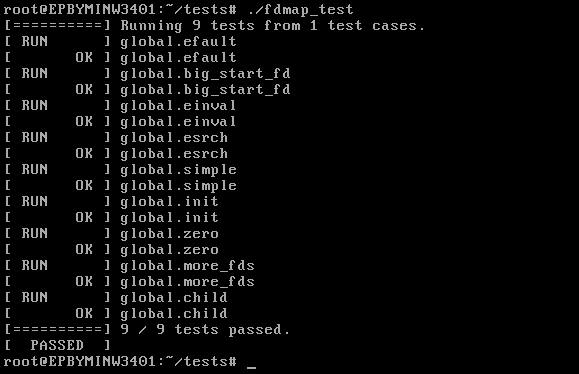
\includegraphics[width=\textwidth]{selftest.png}
  \caption{Результаты работы тестирующей программы}
  \label{fig:selftest}
\end{figure}

Тесты для других системных вызовов организованы по тем же принципам, поэтому не
будем останавливаться на каждом из них подробно. Рассмотрим только те, которые
значительно отличаются от остальных. К таким тестам особенно отличается тест на
отсутствие выходов за пределы выделенной памяти в вызове \texttt{pidfdinfo}. Как
известно, если наличие записи за предел можно проверить непосредственной
проверкой значений, доступа в которые не должно быть (как, например,
осуществляется в SLUB-аллокаторе), то чтение за пределами как правило отследить
значительно сложнее. Поэтому, для точной проверки в тесте применена следующая
схема: вызовом \texttt{mmap()} процесс получает три страницы, расположенные
подряд, при этом две крайние страницы должны иметь флаг защиты
\texttt{PROT\_NONE}, то есть должен предотвращаться любой доступ к памяти, а
центральная страница должна иметь защиту \texttt{PROT\_WRITE} (право только на
запись) или иную в случае проверки иного доступа. Также можно одним системным
вызовом получить три страницы \texttt{PROT\_NONE}, а затем изменить защиту одной
вызовом \texttt{mprotect()}. Данный системный вызов позволяет изменять права на
доступ к страницам. Указатель на страницу среднюю
страницу передается системному вызову в качестве буфера, и если в результате
работы произойдет какой-либо доступ к памяти соседних страниц, сгенерируется
исключение и зафиксируется ошибка Page Fault. Подобная проверка является более
надежной ввиду того, что факт нежелательных действий проверяется аппаратно.
Результат работы собранной тестирующей программы показан на рисунке
\ref{fig:selftest}. Все тесты отрабатывают успешно. Целиком тест выглядит
следующим образом:
\medskip
\begin{lstlisting}[style=cstyle]
TEST(page_edge)
{
	void *page;

	page = mmap(NULL, SIZE * 3, PROT_NONE,
			MAP_PRIVATE | MAP_ANONYMOUS, 0, 0);
	ASSERT_NE(MAP_FAILED, page);
	ASSERT_NE(-1, mprotect(page + SIZE,
			SIZE, PROT_WRITE));
	ASSERT_LT(0, pidfdinfo(0, 1, page + SIZE, SIZE));
	munmap(page, SIZE * 3);
}
\end{lstlisting}
\medskip

Реализация примеров пользовательских программ по своей сути является
демонстрацией использования системных вызовов и их интерфейса, поэтому
использование новых системных вызовов пользовательским пространством будет
рассмотрено в разделе \ref{sec:manual}.
